% !TEX root = ../main.tex

\section{Zlepšenie stavu robota}

\subsection{Chyba v~systéme}
\label{subsec:brokenSystem}

Prvýkrát, keď sme prišli k~robotu do~NCR (\acrlong{NCR}), tak~sme si určili ako prvú úlohu zálohovať systém. Ak~by sa teda stala nejaká chyba
a~robot by prestal fungovať, tak~by sme sa vedeli dostať do~posledného funkčného stavu robota. Zálohovanie systému nanešťastie nebolo možné
hneď po~zapnutí robota. Bolo to~spôsobené poškodeným balíkovým systémom. Tento problém bol zapríčinený nesprávnou
inštaláciou a~následným nesprávnym odstránením ROS1 (\acrlong{ROS}). Verzia, ktorá bola pôvodne nainštalovaná na~robote
bola \textit{Lunar Loggerhead}. Toto by problém nespôsobilo, čo ale~problém spôsobilo, bolo jeho nesprávne odinštalovanie.
Táto akcia mala za~dôsledok vypisovanie nasledovnej chybovej hlášky pri~zálohovaní.

\begin{lstlisting}
	E: Unable to~correct problems, you have held broken packages.
\end{lstlisting}

Tento problém sme vyriešil vymazaním všetkých knižníc, ktoré boli nainštalované spolu s~ROS1. Toto vyriešilo problém. Na~vymazanie týchto
knižníc sme použili nasledovný príkaz.

\begin{lstlisting}[language=bash]
	sudo apt autoremove && sudo dpkg --remove $(dpkg --get-selections | grep hold)
\end{lstlisting}

Tento príkaz najprv odstráni všetky balíčky, ktoré nie sú~používané žiadnou aplikáciu v~systéme. Následne vyhľadá všetky knižnice,
ktoré taktiež nie sú~používané žiadnym balíčkom a~nasilu odinštaluje. Po~vykonaní tejto operácie sme ešte museli odstrániť všetky referencie
na~ROS1 v~systéme. Toto sme vykonali odstránením prepojení na~už~neaktívne repozitáre, ktoré sa nachádzali v~súbore \textit{/etc/apt/sources.list}.

\subsection{Chyba v~dokumentácii}
\label{subsec:documentationIssue}

V~kapitole~\ref{sec:ovladanie} sme uviedli pôvodný stav ovládania robota pomocou správ typu JSON.
Z~kódu~\ref{jsonSpeedRequestBad} je jasné, že~sa majú posielať celé čísla a~na~základe tohto vstupu sa bude robot hýbať. Čo sme zistili až
po~skompilovaní a~spustení tímového projektu je, že~sa majú posielať desatinné čísla z~intervalu 0 až 1. Toto nebolo písané
v~dokumentácii, ktorá nám bola dodaná na~začiatku programu. Môžeme preto~príklad prepísať na~reťazec, ktorý by fungoval:

	\label{jsonSpeedRequestGood}
	\begin{lstlisting}
			{"UserID":1,"Command":3,"RightWheelSpeed":0.50,"LeftWheelSpeed":0.50}
	\end{lstlisting}

\subsection{Oneskorenie komunikácie}
\label{subsec:communicationDelay}

Pri~blízkom pohľade na~kód robota sme odhalili závažnú chybu. Vo~vlákne, ktoré zabezpečuje prijímanie správ sa nachádza
cyklus, ktorý prijíma dáta z~TCP/IP spojenia a~bezpečne ich zapisuje do~zdielanej štruktúry. Prijímanie správ je realizované
pomocou funkcie \textit{recv} z~knižnice \textit{sys/socket.h}. Táto funkcia je za~normálach podmienok blokujúca, to~znamená,
že~vlákno, ktoré ju volá, sa zablokuje, až pokým nemá k~dispozícii dáta na~čítanie. Na~robote je toto blokovanie
vypnutý s~tým že~po~každom zavolaní tejto funkcie sa čaká \textit{100 milisekúnd}. Tento problém je ľahko opraviteľný.
Čo sme spravili bolo, že~sme odstránili funkciu \textit{usleep}, ktorá zabezpečovala čakanie. Vo~funkcii \textit{recv}
sme ďalej vymazali makro \textit{MSG\_DONTWAIT}, ktoré spôsobuje, že~sa funkcia \textit{recv} nezablokovala.

\subsection{Rozšírenie príkazov robota}
\label{subsec:extendRobotCommands}

Prvotne sme mali v~plane získavať pozíciu robota pomocou príkazov, ktoré sa nachádzajú v~knižnici enkóderov.
Tieto príkazy mali vracať počet impulzov IRC snímačov prejdených od~spustenia robota.
Pre~zaobchádzanie s~touto funkcionalitou sme definovali dva príkazy:\\

\noindent \textbf{Command:~\ref{c4}} \\
\indent Tento príkaz je prázdny. My sme ho ale~neskôr prepísali na~príkaz, cez~ktorý sa dá nastaviť
žiadaná pozícia kolies robota (ich natočenie) pomocou funkcii z~kniznice EPOS \cite{EPOSdoc}.
Táto funkcionalita nie je v~takom stave ako sme si priali. Je to~spôsobené hlavne nepostačujúcou dokumentáciou enkóderov na~robote. Síce sme našli
v~dokumentácii funkciu, ktorá by mala túto možnosť povoľovať. Čo sa ale~stane pri~poslaní príkazu je to, že~kolesá sa začnú točiť rýchlosťou
0,5 metra za~sekundu.\\

\noindent \textbf{Command:~\ref{c8}} \\
\indent Príkaz na~zisťovanie polohy kolies nebol pôvodne naprogramovaný na~robote. Pridali sme ho za~cieľom presného
dostavenia sa robota na~preddefinované miesto. Táto funkcionalita nefunguje správne rovnako ako v~predchádzajúcom príklade,
keď si vypýtame polohu kolies od~robota, dáta ktoré obdržme sú, že~jedno koleso je priamo nastavené na~hodnotu, ktorú sme si
vyžiadali a~to~druhé koleso vráti náhodnú hodnotu. Počas toho sa ale~kolesá robota stále točia.\\

Tento postup sa ukázal ako neuskutočniteľný, lebo príkazom~\ref{c8} sme z~jedného enkódery
získavali informácie priamo nastavenej polohy a~z~druhého enkódera sme dodržiavali čisto náhodné dáta.
Z~tohto dôvodu sme sa rozhodli využívať spätnú väzbu, ktorá obsahuje rýchlosti robota.

\clearpage

\subsection{Nesprávna spätná väzba}
\label{subsec:wrongFeedback}

Ako bolo spomenuté vyššie, pri~poslaní príkazu s~číslom~\ref{c6} nám robot vráti aktuálne rýchlosti kolies. Počas skúšania tejto funkcionality
sme narazili na~problém. Keď sme sa robota spýtali na~jeho rýchlosti. Dostali sme reťazec, ktorý obsahoval náhodne veľké čísla. Tieto čísla sa
menili, keď sme zadávali nejaké hodnoty pre~rýchlosti kolies aby~sa robot hýbal. Ich magnitúda ale~ostávala nezmenená. V~nasledujúcom príklade
môžeme vidieť ako tento reťazec vyzeral:

\label{jsonWannabeSpeed}
\begin{lstlisting}
		{"LeftWheelSpeed"=236223201280 "RightWheelSpeed"=4294967296}
\end{lstlisting}

Ako si môžeme všimnúť. Pri~tomto type správ nie je dodržaná správna forma reťazca typu \textit{JSON}.
Namiesto `:' máme `=' a~medzi argumentmi sa nenachádza čiarka. Hneď ako prvú vec sme chceli tento štandard napraviť. Bohužiaľ na~tomto
robote už~bolo spravených niekoľko projektov a~museli by sme prejsť každý z~nich a~zistiť či~používajú túto spätnú väzbu. Ak~by ju používali
museli by sme tieto kódy upraviť.

V~dokumentácii robota bohužiaľ nebolo písané v~akom formáte sa tieto rýchlosti kolies majú nachádzať. Preto~jeden z~nápadov ako zistiť presne
v~akom formáte sa posielali tieto čísla bolo vyskúšať pár možností:

\begin{itemize}
	\item \textit{long} - celé číslo s~malým endianom
	\item \textit{long} - celé číslo s~veľkým endianom
	\item \textit{float} - desatinné číslo s~malým endianom
	\item \textit{float} - desatinné číslo s~veľkým endianom
\end{itemize}

Keďže robot má počítač so~64 bytovým procesorom \cite{robotPc}, tak~\textit{long} aj~\textit{float} budú mať 64 bitovú dĺžku. Po~skúsení všetkých
štyroch možností sa~ukázalo, že~ani jedna nebola správna a~problém je niekde inde.

Aby sme pochopili, ako sa máme správať k~prijatým dátam musíme vedieť ako funguje program na~robote.
Skopírovali sme si preto~kód z~robota a~pustili sme sa do~jeho analýzy. Pri~poslaní požiadavky
na~nastavenie rýchlostí kolies si ich robot premení na~celé čísla v~rozsahu 0~až~1000. To~je hodnota, na~ktorú nastaví
rýchlosti otáčania pravého a~ľavého kolesa respektíve rýchlosť otáčania ich motorov. Na~druhú stranu,
keď si vypýtame od~robota rýchlosti kolies. On zoberie informáciu z~enkóderov a~pošle nám ju~bez spracovania. Aj~napriek týmto poznatkom sa nám
nepodarilo získať z~týchto dát žiadané rýchlosti.

Po~dôkladnom preštudovaní kódu sme zistili, že~hodnoty ktoré nám posiela robot nie sú~ani~vyťahované z~enkóderov správnou funkciou. Preto~sme ju
zmenili a~začali sme dostávať hodnoty, s~ktorými by sa mohlo dať pracovať.

Funkcie z~knižnice zabezpečujúce komunikáciu z~enkóderov motorov pochádzajú z~firmy Maxon~\cite{EPOSdoc}. Táto dokumentácia nebola moc nápomocná.
Opisy jednotlivých funkcií boli len~ich rozložené názvy na~osobitné slová. Aj~napriek tomu sa nám podarilo nájsť funkcie, ktoré sme potrebovali.
Funkcie obsahujúce slovo `Target', majú návratné hodnoty reprezentujúce žiadané hodnoty. Funkcie s~príponou
`-Is' vracajú aktuálne hodnoty. Z~tohto dôvodu sme museli prepísať funkciu na~robote, ktorá sa vykonávala.
Pre~získanie aktuálnych hodnôt rýchlosti motora poslaním príkazu \ref{c6} sme museli zmeniť nasledujúcu funkciu:

\lstset{language=C++,
	basicstyle=\ttfamily,
	keywordstyle=\color{blue}\ttfamily,
	stringstyle=\color{red}\ttfamily,
	commentstyle=\color{green}\ttfamily,
	morecomment=[l][\color{magenta}]{\#},
	numberstyle=\color{orange}
}

\label{VelocityIs}
\begin{lstlisting}[language=C++]
BOOL VCS_GetTargetVelocity(
	HANDLE KeyHandle,
	WORD NodeId,
	long* pTargetVelocity,
	DWORD* pErrorCode);
\end{lstlisting}

\begin{lstlisting}[language=C++]
BOOL VCS_GetVelocityIs(
	HANDLE KeyHandle,
	WORD NodeId,
	long* pVelocityIs,
	DWORD* pErrorCode);
\end{lstlisting}

\noindent Ako môžeme vidieť v~týchto predpisoch funkcií, bolo treba zmeniť názov funkcie a~ostatné parametre ostali rovnaké.
Nebolo treba meniť implementáciu kódu.

\subsection{Zašumený výstup}
\label{subsec:outputNoice}

Po~prepísaní funkcie na~získavanie rýchlostí robota sme spravili pár meraní, aby sme zistili,
aké presné informácie o~rýchlostiach motorov dostávame. Vykonali sme meranie prechodovej a~prevodovej charakteristiky
oboch motorov, tým, že~bol zabezpečený pohyb kolies vo~vzduchu s~vypodložením robota.

\begin{figure}[!htbp]
	\begin{subfigure}{0.5\textwidth}
		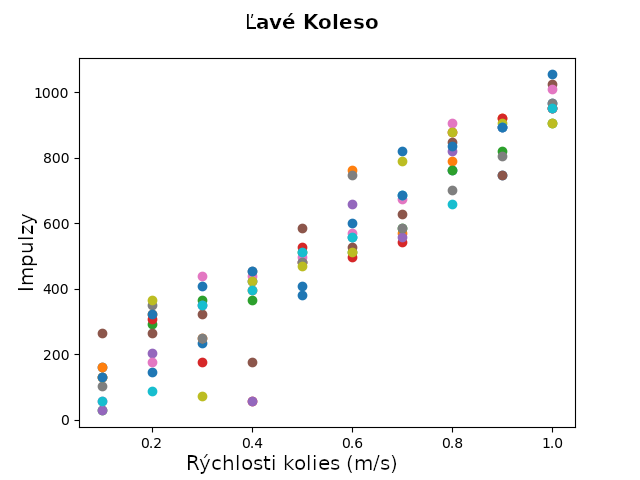
\includegraphics[width=\textwidth]{img/Left_wheel_2.png}
	\end{subfigure}
	\hfill
	\begin{subfigure}{0.5\textwidth}
		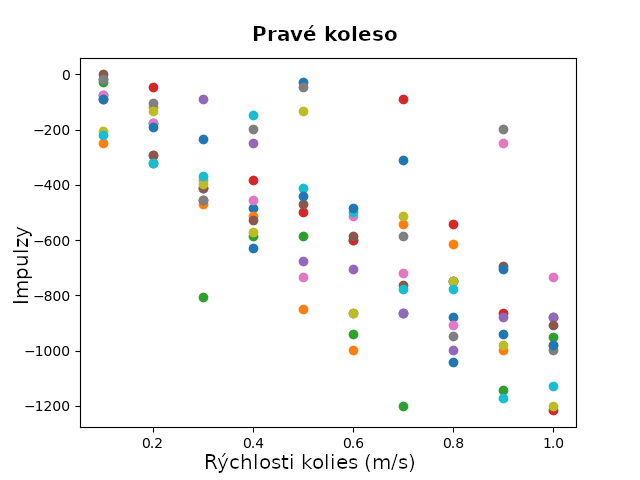
\includegraphics[width=\textwidth]{img/Right_wheel_2.png}
	\end{subfigure}
	\caption{Ustálené hodnoty rýchlosti ľavého a~pravého motora. }
	\label{fig:lavePraveKoleso}
\end{figure}

Na~obrázku Obr.~\ref{fig:prechChar} vidíme zašmený signál rýchlostí, ktoré sme obdržali z~enkóderov. Predpokladá sa,
že~toto zašumenie je spôsobené nesprávnym vedením káblov robota, prípadne nepostačujúcim izolovaním ich niektorých
častí. Keď sa pozrieme na~obrázok Obr.~\ref{fig:robot}, tak~môžeme vidieť nesprávny manažment káblov. Túto teóriu
potvrdzuje aj~fakt, že~spätná väzba rýchlosti, keď robot stojí neobsahuje rušenie a~je zaručene 0. Problémy zo~zašmeným
signálom riešili aj~už~v~spomínanom tímovom projekte~\cite{timovyProjekt}. Im sa podarilo spraviť graf prechodovej
charakteristiky rýchlosti kolies zobrazený na~Obr.~\ref{fig:prechChar}.

\begin{figure}[!htbp]
	\begin{center}
		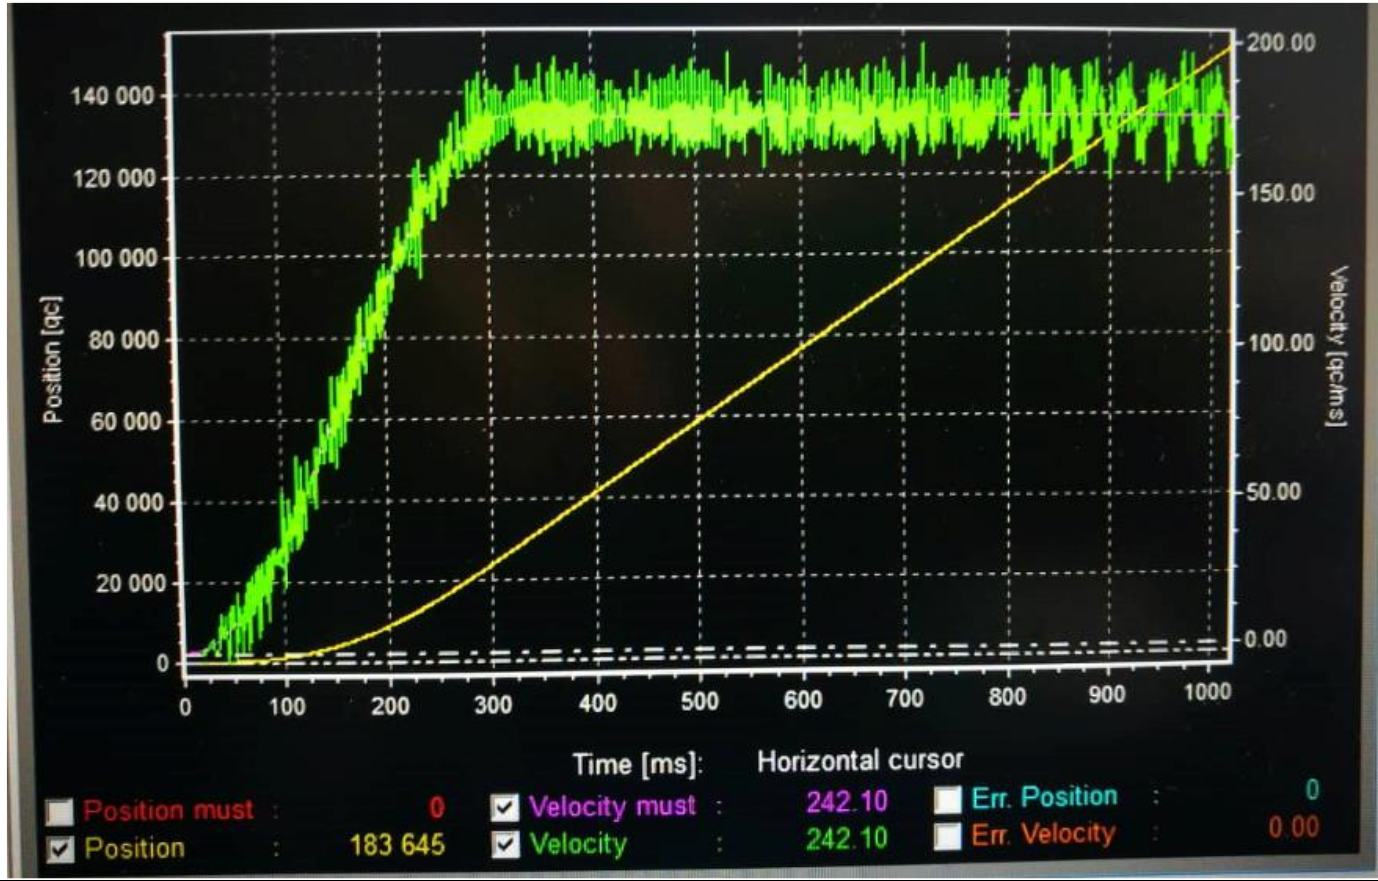
\includegraphics[width=0.95\textwidth]{img/robotSpeedChar.png}
	\end{center}
	\caption{Prechodová charakteristika rýchlosti kolies~\cite{timovyProjekt}. }
	\label{fig:prechChar}
\end{figure}

\clearpage
